\documentclass[1p]{elsarticle_modified}
%\bibliographystyle{elsarticle-num}

%\usepackage[colorlinks]{hyperref}
%\usepackage{abbrmath_seonhwa} %\Abb, \Ascr, \Acal ,\Abf, \Afrak
\usepackage{amsfonts}
\usepackage{amssymb}
\usepackage{amsmath}
\usepackage{amsthm}
\usepackage{scalefnt}
\usepackage{amsbsy}
\usepackage{kotex}
\usepackage{caption}
\usepackage{subfig}
\usepackage{color}
\usepackage{graphicx}
\usepackage{xcolor} %% white, black, red, green, blue, cyan, magenta, yellow
\usepackage{float}
\usepackage{setspace}
\usepackage{hyperref}

\usepackage{tikz}
\usetikzlibrary{arrows}

\usepackage{multirow}
\usepackage{array} % fixed length table
\usepackage{hhline}

%%%%%%%%%%%%%%%%%%%%%
\makeatletter
\renewcommand*\env@matrix[1][\arraystretch]{%
	\edef\arraystretch{#1}%
	\hskip -\arraycolsep
	\let\@ifnextchar\new@ifnextchar
	\array{*\c@MaxMatrixCols c}}
\makeatother %https://tex.stackexchange.com/questions/14071/how-can-i-increase-the-line-spacing-in-a-matrix
%%%%%%%%%%%%%%%

\usepackage[normalem]{ulem}

\newcommand{\msout}[1]{\ifmmode\text{\sout{\ensuremath{#1}}}\else\sout{#1}\fi}
%SOURCE: \msout is \stkout macro in https://tex.stackexchange.com/questions/20609/strikeout-in-math-mode

\newcommand{\cancel}[1]{
	\ifmmode
	{\color{red}\msout{#1}}
	\else
	{\color{red}\sout{#1}}
	\fi
}

\newcommand{\add}[1]{
	{\color{blue}\uwave{#1}}
}

\newcommand{\replace}[2]{
	\ifmmode
	{\color{red}\msout{#1}}{\color{blue}\uwave{#2}}
	\else
	{\color{red}\sout{#1}}{\color{blue}\uwave{#2}}
	\fi
}

\newcommand{\Sol}{\mathcal{S}} %segment
\newcommand{\D}{D} %diagram
\newcommand{\A}{\mathcal{A}} %arc


%%%%%%%%%%%%%%%%%%%%%%%%%%%%%5 test

\def\sl{\operatorname{\textup{SL}}(2,\Cbb)}
\def\psl{\operatorname{\textup{PSL}}(2,\Cbb)}
\def\quan{\mkern 1mu \triangleright \mkern 1mu}

\theoremstyle{definition}
\newtheorem{thm}{Theorem}[section]
\newtheorem{prop}[thm]{Proposition}
\newtheorem{lem}[thm]{Lemma}
\newtheorem{ques}[thm]{Question}
\newtheorem{cor}[thm]{Corollary}
\newtheorem{defn}[thm]{Definition}
\newtheorem{exam}[thm]{Example}
\newtheorem{rmk}[thm]{Remark}
\newtheorem{alg}[thm]{Algorithm}

\newcommand{\I}{\sqrt{-1}}
\begin{document}

%\begin{frontmatter}
%
%\title{Boundary parabolic representations of knots up to 8 crossings}
%
%%% Group authors per affiliation:
%\author{Yunhi Cho} 
%\address{Department of Mathematics, University of Seoul, Seoul, Korea}
%\ead{yhcho@uos.ac.kr}
%
%
%\author{Seonhwa Kim} %\fnref{s_kim}}
%\address{Center for Geometry and Physics, Institute for Basic Science, Pohang, 37673, Korea}
%\ead{ryeona17@ibs.re.kr}
%
%\author{Hyuk Kim}
%\address{Department of Mathematical Sciences, Seoul National University, Seoul 08826, Korea}
%\ead{hyukkim@snu.ac.kr}
%
%\author{Seokbeom Yoon}
%\address{Department of Mathematical Sciences, Seoul National University, Seoul, 08826,  Korea}
%\ead{sbyoon15@snu.ac.kr}
%
%\begin{abstract}
%We find all boundary parabolic representation of knots up to 8 crossings.
%
%\end{abstract}
%\begin{keyword}
%    \MSC[2010] 57M25 
%\end{keyword}
%
%\end{frontmatter}

%\linenumbers
%\tableofcontents
%
\newcommand\colored[1]{\textcolor{white}{\rule[-0.35ex]{0.8em}{1.4ex}}\kern-0.8em\color{red} #1}%
%\newcommand\colored[1]{\textcolor{white}{ #1}\kern-2.17ex	\textcolor{white}{ #1}\kern-1.81ex	\textcolor{white}{ #1}\kern-2.15ex\color{red}#1	}

{\Large $\underline{12a_{0622}~(K12a_{0622})}$}

\setlength{\tabcolsep}{10pt}
\renewcommand{\arraystretch}{1.6}
\vspace{1cm}\begin{tabular}{m{100pt}>{\centering\arraybackslash}m{274pt}}
\multirow{5}{120pt}{
	\centering
	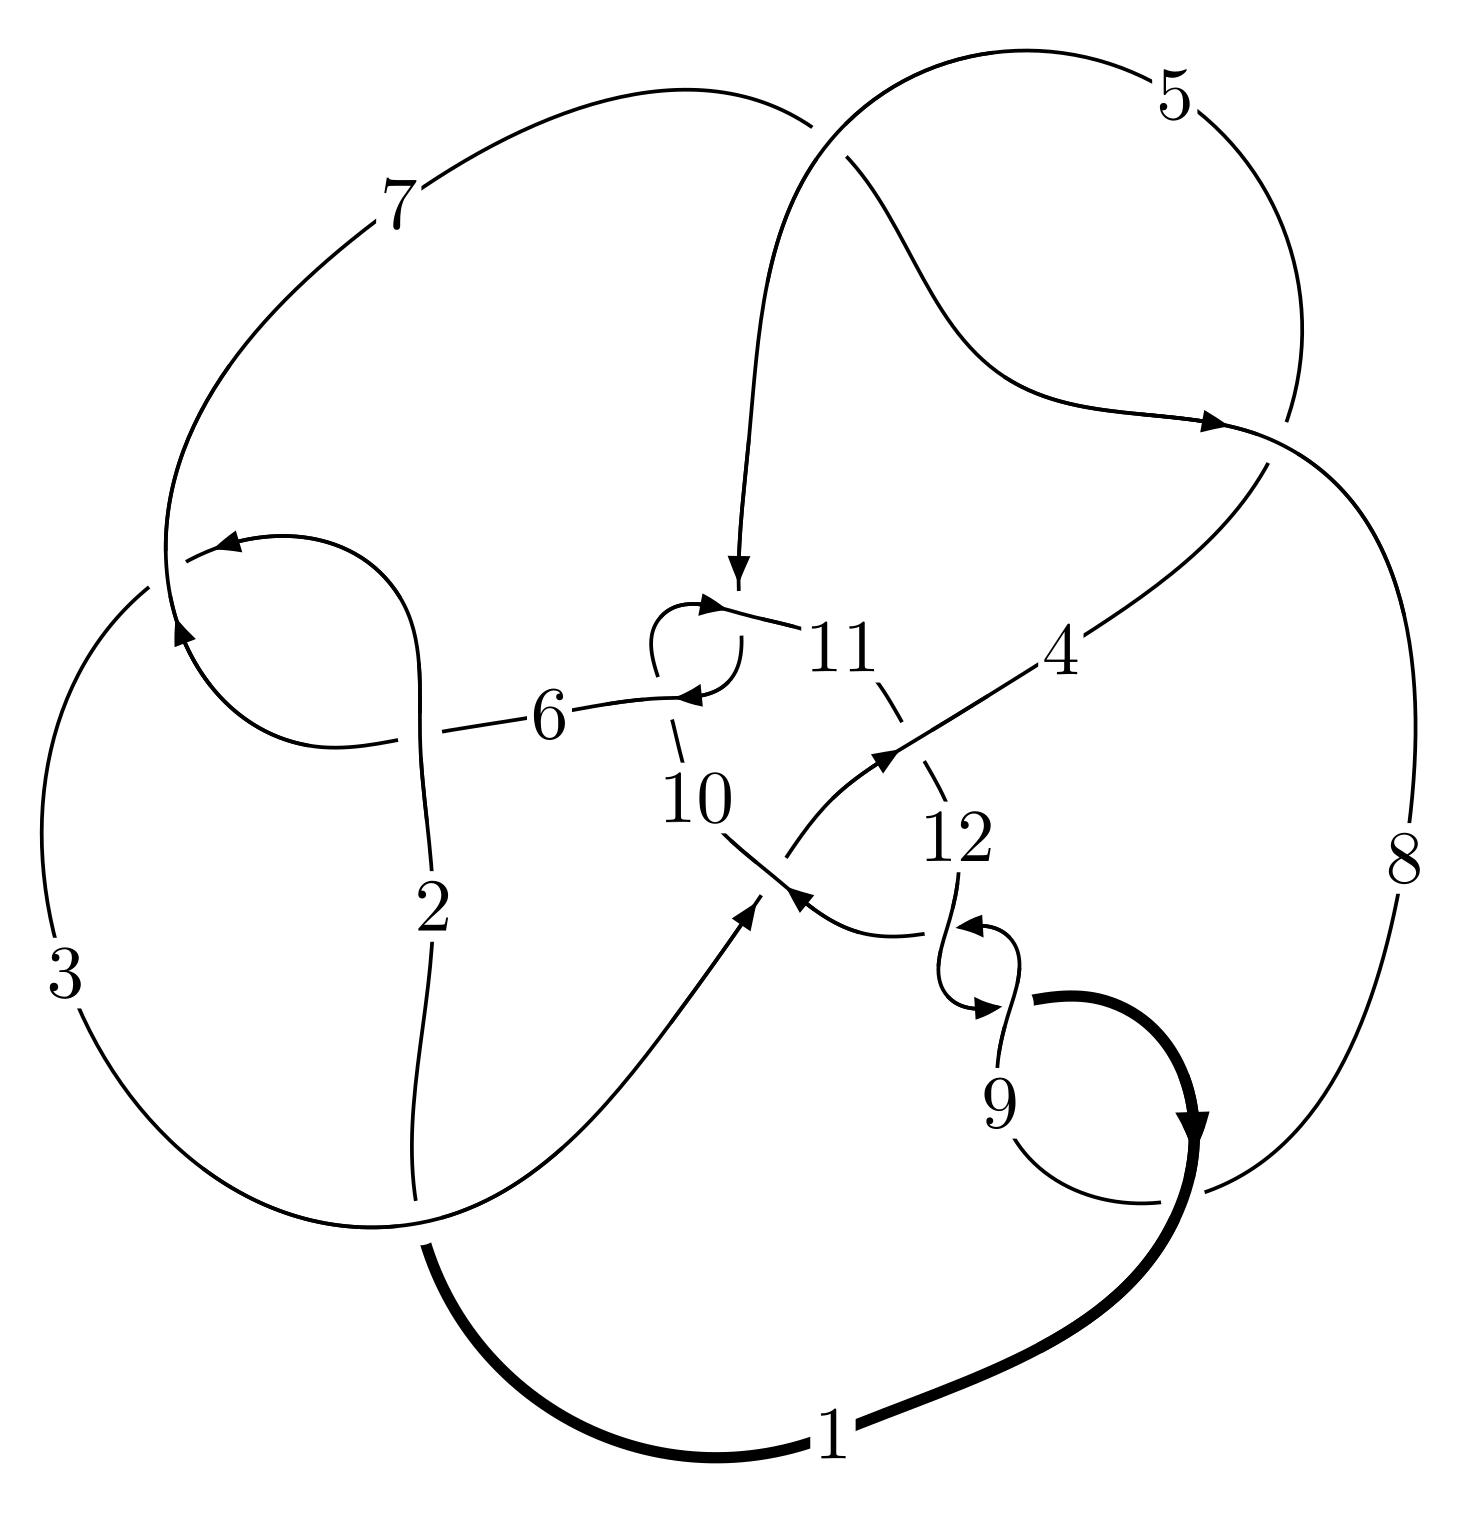
\includegraphics[width=112pt]{../../../GIT/diagram.site/Diagrams/png/1423_12a_0622.png}\\
\ \ \ A knot diagram\footnotemark}&
\allowdisplaybreaks
\textbf{Linearized knot diagam} \\
\cline{2-2}
 &
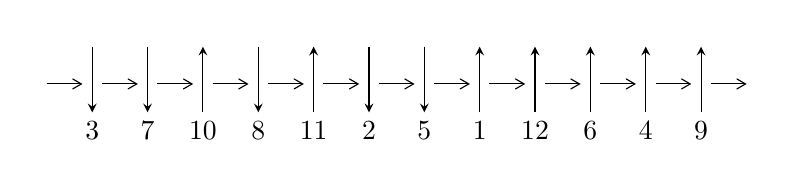
\begin{tikzpicture}[x=20pt, y=17pt]
	% nodes
	\node (C0) at (0, 0) {};
	\node (C1) at (1, 0) {};
	\node (C1U) at (1, +1) {};
	\node (C1D) at (1, -1) {3};

	\node (C2) at (2, 0) {};
	\node (C2U) at (2, +1) {};
	\node (C2D) at (2, -1) {7};

	\node (C3) at (3, 0) {};
	\node (C3U) at (3, +1) {};
	\node (C3D) at (3, -1) {10};

	\node (C4) at (4, 0) {};
	\node (C4U) at (4, +1) {};
	\node (C4D) at (4, -1) {8};

	\node (C5) at (5, 0) {};
	\node (C5U) at (5, +1) {};
	\node (C5D) at (5, -1) {11};

	\node (C6) at (6, 0) {};
	\node (C6U) at (6, +1) {};
	\node (C6D) at (6, -1) {2};

	\node (C7) at (7, 0) {};
	\node (C7U) at (7, +1) {};
	\node (C7D) at (7, -1) {5};

	\node (C8) at (8, 0) {};
	\node (C8U) at (8, +1) {};
	\node (C8D) at (8, -1) {1};

	\node (C9) at (9, 0) {};
	\node (C9U) at (9, +1) {};
	\node (C9D) at (9, -1) {12};

	\node (C10) at (10, 0) {};
	\node (C10U) at (10, +1) {};
	\node (C10D) at (10, -1) {6};

	\node (C11) at (11, 0) {};
	\node (C11U) at (11, +1) {};
	\node (C11D) at (11, -1) {4};

	\node (C12) at (12, 0) {};
	\node (C12U) at (12, +1) {};
	\node (C12D) at (12, -1) {9};
	\node (C13) at (13, 0) {};

	% arrows
	\draw[->,>={angle 60}]
	(C0) edge (C1) (C1) edge (C2) (C2) edge (C3) (C3) edge (C4) (C4) edge (C5) (C5) edge (C6) (C6) edge (C7) (C7) edge (C8) (C8) edge (C9) (C9) edge (C10) (C10) edge (C11) (C11) edge (C12) (C12) edge (C13) ;	\draw[->,>=stealth]
	(C1U) edge (C1D) (C2U) edge (C2D) (C3D) edge (C3U) (C4U) edge (C4D) (C5D) edge (C5U) (C6U) edge (C6D) (C7U) edge (C7D) (C8D) edge (C8U) (C9D) edge (C9U) (C10D) edge (C10U) (C11D) edge (C11U) (C12D) edge (C12U) ;
	\end{tikzpicture} \\
\hhline{~~} \\& 
\textbf{Solving Sequence} \\ \cline{2-2} 
 &
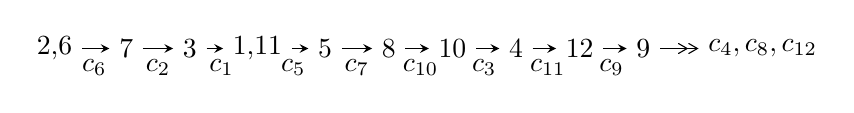
\begin{tikzpicture}[x=23pt, y=7pt]
	% node
	\node (A0) at (-1/8, 0) {2,6};
	\node (A1) at (1, 0) {7};
	\node (A2) at (2, 0) {3};
	\node (A3) at (49/16, 0) {1,11};
	\node (A4) at (33/8, 0) {5};
	\node (A5) at (41/8, 0) {8};
	\node (A6) at (49/8, 0) {10};
	\node (A7) at (57/8, 0) {4};
	\node (A8) at (65/8, 0) {12};
	\node (A9) at (73/8, 0) {9};
	\node (C1) at (1/2, -1) {$c_{6}$};
	\node (C2) at (3/2, -1) {$c_{2}$};
	\node (C3) at (5/2, -1) {$c_{1}$};
	\node (C4) at (29/8, -1) {$c_{5}$};
	\node (C5) at (37/8, -1) {$c_{7}$};
	\node (C6) at (45/8, -1) {$c_{10}$};
	\node (C7) at (53/8, -1) {$c_{3}$};
	\node (C8) at (61/8, -1) {$c_{11}$};
	\node (C9) at (69/8, -1) {$c_{9}$};
	\node (A10) at (11, 0) {$c_{4},c_{8},c_{12}$};

	% edge
	\draw[->,>=stealth]	
	(A0) edge (A1) (A1) edge (A2) (A2) edge (A3) (A3) edge (A4) (A4) edge (A5) (A5) edge (A6) (A6) edge (A7) (A7) edge (A8) (A8) edge (A9) ;
	\draw[->>,>={angle 60}]	
	(A9) edge (A10);
\end{tikzpicture} \\ 

\end{tabular} \\

\footnotetext{
The image of knot diagram is generated by the software ``\textbf{Draw programme}" developed by Andrew Bartholomew(\url{http://www.layer8.co.uk/maths/draw/index.htm\#Running-draw}), where we modified some parts for our purpose(\url{https://github.com/CATsTAILs/LinksPainter}).
}\phantom \\ \newline 
\centering \textbf{Ideals for irreducible components\footnotemark of $X_{\text{par}}$} 
 
\begin{align*}
I^u_{1}&=\langle 
4.48195\times10^{360} u^{129}-2.24649\times10^{360} u^{128}+\cdots+1.41689\times10^{360} b-1.72726\times10^{363},\\
\phantom{I^u_{1}}&\phantom{= \langle  }4.29505\times10^{363} u^{129}-5.66837\times10^{362} u^{128}+\cdots+3.98147\times10^{362} a-1.19128\times10^{366},\\
\phantom{I^u_{1}}&\phantom{= \langle  }u^{130}- u^{129}+\cdots-2132 u+281\rangle \\
I^u_{2}&=\langle 
16 u^{31}-6 u^{30}+\cdots+b+17,\;-36 u^{31}+35 u^{30}+\cdots+a-60,\;u^{32}-8 u^{30}+\cdots+3 u+1\rangle \\
\\
\end{align*}
\raggedright * 2 irreducible components of $\dim_{\mathbb{C}}=0$, with total 162 representations.\\
\footnotetext{All coefficients of polynomials are rational numbers. But the coefficients are sometimes approximated in decimal forms when there is not enough margin.}
\newpage
\renewcommand{\arraystretch}{1}
\centering \section*{I. $I^u_{1}= \langle 4.48\times10^{360} u^{129}-2.25\times10^{360} u^{128}+\cdots+1.42\times10^{360} b-1.73\times10^{363},\;4.30\times10^{363} u^{129}-5.67\times10^{362} u^{128}+\cdots+3.98\times10^{362} a-1.19\times10^{366},\;u^{130}- u^{129}+\cdots-2132 u+281 \rangle$}
\flushleft \textbf{(i) Arc colorings}\\
\begin{tabular}{m{7pt} m{180pt} m{7pt} m{180pt} }
\flushright $a_{2}=$&$\begin{pmatrix}0\\u\end{pmatrix}$ \\
\flushright $a_{6}=$&$\begin{pmatrix}1\\0\end{pmatrix}$ \\
\flushright $a_{7}=$&$\begin{pmatrix}1\\u^2\end{pmatrix}$ \\
\flushright $a_{3}=$&$\begin{pmatrix}- u\\- u^3+u\end{pmatrix}$ \\
\flushright $a_{1}=$&$\begin{pmatrix}u^3\\u^5- u^3+u\end{pmatrix}$ \\
\flushright $a_{11}=$&$\begin{pmatrix}-10.7876 u^{129}+1.42369 u^{128}+\cdots-20220.3 u+2992.06\\-3.16322 u^{129}+1.58550 u^{128}+\cdots-7878.65 u+1219.05\end{pmatrix}$ \\
\flushright $a_{5}=$&$\begin{pmatrix}-0.320480 u^{129}-1.28783 u^{128}+\cdots+1797.24 u-334.920\\-1.64933 u^{129}-1.18720 u^{128}+\cdots-695.804 u+38.0681\end{pmatrix}$ \\
\flushright $a_{8}=$&$\begin{pmatrix}-5.51277 u^{129}+0.141240 u^{128}+\cdots-9094.61 u+1307.14\\-3.33741 u^{129}+1.09015 u^{128}+\cdots-7233.58 u+1092.81\end{pmatrix}$ \\
\flushright $a_{10}=$&$\begin{pmatrix}-7.62437 u^{129}-0.161817 u^{128}+\cdots-12341.7 u+1773.01\\-3.16322 u^{129}+1.58550 u^{128}+\cdots-7878.65 u+1219.05\end{pmatrix}$ \\
\flushright $a_{4}=$&$\begin{pmatrix}-1.53534 u^{129}-1.41287 u^{128}+\cdots+106.463 u-101.642\\-2.45838 u^{129}-0.606476 u^{128}+\cdots-2961.13 u+391.626\end{pmatrix}$ \\
\flushright $a_{12}=$&$\begin{pmatrix}-1.29895 u^{129}-0.443172 u^{128}+\cdots-1206.94 u+133.828\\0.770830 u^{129}-0.0309308 u^{128}+\cdots+1333.06 u-193.571\end{pmatrix}$ \\
\flushright $a_{9}=$&$\begin{pmatrix}-3.29734 u^{129}-0.470625 u^{128}+\cdots-4505.06 u+619.044\\-2.55890 u^{129}+0.952322 u^{128}+\cdots-5780.28 u+879.275\end{pmatrix}$\\&\end{tabular}
\flushleft \textbf{(ii) Obstruction class $= -1$}\\~\\
\flushleft \textbf{(iii) Cusp Shapes $= 9.85019 u^{129}-2.86707 u^{128}+\cdots+21034.7 u-3194.45$}\\~\\
\newpage\renewcommand{\arraystretch}{1}
\flushleft \textbf{(iv) u-Polynomials at the component}\newline \\
\begin{tabular}{m{50pt}|m{274pt}}
Crossings & \hspace{64pt}u-Polynomials at each crossing \\
\hline $$\begin{aligned}c_{1}\end{aligned}$$&$\begin{aligned}
&u^{130}+59 u^{129}+\cdots+2798166 u+78961
\end{aligned}$\\
\hline $$\begin{aligned}c_{2},c_{6}\end{aligned}$$&$\begin{aligned}
&u^{130}- u^{129}+\cdots-2132 u+281
\end{aligned}$\\
\hline $$\begin{aligned}c_{3}\end{aligned}$$&$\begin{aligned}
&u^{130}+17 u^{128}+\cdots+693261 u+67289
\end{aligned}$\\
\hline $$\begin{aligned}c_{4},c_{7}\end{aligned}$$&$\begin{aligned}
&u^{130}-4 u^{129}+\cdots-77445 u+8257
\end{aligned}$\\
\hline $$\begin{aligned}c_{5},c_{10}\end{aligned}$$&$\begin{aligned}
&u^{130}+u^{129}+\cdots+u+1
\end{aligned}$\\
\hline $$\begin{aligned}c_{8},c_{9},c_{12}\end{aligned}$$&$\begin{aligned}
&u^{130}+3 u^{129}+\cdots+167 u+49
\end{aligned}$\\
\hline $$\begin{aligned}c_{11}\end{aligned}$$&$\begin{aligned}
&u^{130}-5 u^{129}+\cdots+300381 u+21815
\end{aligned}$\\
\hline
\end{tabular}\\~\\
\newpage\renewcommand{\arraystretch}{1}
\flushleft \textbf{(v) Riley Polynomials at the component}\newline \\
\begin{tabular}{m{50pt}|m{274pt}}
Crossings & \hspace{64pt}Riley Polynomials at each crossing \\
\hline $$\begin{aligned}c_{1}\end{aligned}$$&$\begin{aligned}
&y^{130}+41 y^{129}+\cdots+2849686224134 y+6234839521
\end{aligned}$\\
\hline $$\begin{aligned}c_{2},c_{6}\end{aligned}$$&$\begin{aligned}
&y^{130}-59 y^{129}+\cdots-2798166 y+78961
\end{aligned}$\\
\hline $$\begin{aligned}c_{3}\end{aligned}$$&$\begin{aligned}
&y^{130}+34 y^{129}+\cdots+179177883001 y+4527809521
\end{aligned}$\\
\hline $$\begin{aligned}c_{4},c_{7}\end{aligned}$$&$\begin{aligned}
&y^{130}+82 y^{129}+\cdots+573275145 y+68178049
\end{aligned}$\\
\hline $$\begin{aligned}c_{5},c_{10}\end{aligned}$$&$\begin{aligned}
&y^{130}+73 y^{129}+\cdots+39 y+1
\end{aligned}$\\
\hline $$\begin{aligned}c_{8},c_{9},c_{12}\end{aligned}$$&$\begin{aligned}
&y^{130}+125 y^{129}+\cdots-124811 y+2401
\end{aligned}$\\
\hline $$\begin{aligned}c_{11}\end{aligned}$$&$\begin{aligned}
&y^{130}+25 y^{129}+\cdots+54768666299 y+475894225
\end{aligned}$\\
\hline
\end{tabular}\\~\\
\newpage\flushleft \textbf{(vi) Complex Volumes and Cusp Shapes}
$$\begin{array}{c|c|c}  
\text{Solutions to }I^u_{1}& \I (\text{vol} + \sqrt{-1}CS) & \text{Cusp shape}\\
 \hline 
\begin{aligned}
u &= -0.918333 + 0.376916 I \\
a &= \phantom{-}0.61362 - 3.16082 I \\
b &= -0.326161 - 1.144000 I\end{aligned}
 & -2.48560 + 3.18878 I & \phantom{-0.000000 } 0 \\ \hline\begin{aligned}
u &= -0.918333 - 0.376916 I \\
a &= \phantom{-}0.61362 + 3.16082 I \\
b &= -0.326161 + 1.144000 I\end{aligned}
 & -2.48560 - 3.18878 I & \phantom{-0.000000 } 0 \\ \hline\begin{aligned}
u &= \phantom{-}1.007430 + 0.080772 I \\
a &= -0.114771 - 0.697783 I \\
b &= \phantom{-}0.783850 + 0.365345 I\end{aligned}
 & -6.62927 + 5.20669 I & \phantom{-0.000000 } 0 \\ \hline\begin{aligned}
u &= \phantom{-}1.007430 - 0.080772 I \\
a &= -0.114771 + 0.697783 I \\
b &= \phantom{-}0.783850 - 0.365345 I\end{aligned}
 & -6.62927 - 5.20669 I & \phantom{-0.000000 } 0 \\ \hline\begin{aligned}
u &= \phantom{-}0.910730 + 0.378156 I \\
a &= \phantom{-}2.08409 + 1.71073 I \\
b &= -0.088955 + 0.742570 I\end{aligned}
 & \phantom{-}0.071473 + 0.583839 I & \phantom{-0.000000 } 0 \\ \hline\begin{aligned}
u &= \phantom{-}0.910730 - 0.378156 I \\
a &= \phantom{-}2.08409 - 1.71073 I \\
b &= -0.088955 - 0.742570 I\end{aligned}
 & \phantom{-}0.071473 - 0.583839 I & \phantom{-0.000000 } 0 \\ \hline\begin{aligned}
u &= \phantom{-}0.414089 + 0.927045 I \\
a &= -0.100985 + 0.378022 I \\
b &= \phantom{-}0.660024 + 1.192480 I\end{aligned}
 & \phantom{-}2.14149 + 8.42500 I & \phantom{-0.000000 } 0 \\ \hline\begin{aligned}
u &= \phantom{-}0.414089 - 0.927045 I \\
a &= -0.100985 - 0.378022 I \\
b &= \phantom{-}0.660024 - 1.192480 I\end{aligned}
 & \phantom{-}2.14149 - 8.42500 I & \phantom{-0.000000 } 0 \\ \hline\begin{aligned}
u &= \phantom{-}0.903721 + 0.388996 I \\
a &= -0.99899 - 2.08540 I \\
b &= -0.14557 - 1.65453 I\end{aligned}
 & -4.38247 - 1.58999 I & \phantom{-0.000000 } 0 \\ \hline\begin{aligned}
u &= \phantom{-}0.903721 - 0.388996 I \\
a &= -0.99899 + 2.08540 I \\
b &= -0.14557 + 1.65453 I\end{aligned}
 & -4.38247 + 1.58999 I & \phantom{-0.000000 } 0\\
 \hline 
 \end{array}$$\newpage$$\begin{array}{c|c|c}  
\text{Solutions to }I^u_{1}& \I (\text{vol} + \sqrt{-1}CS) & \text{Cusp shape}\\
 \hline 
\begin{aligned}
u &= -0.741954 + 0.706883 I \\
a &= -0.521732 - 0.760102 I \\
b &= \phantom{-}0.495114 - 1.034270 I\end{aligned}
 & -2.27849 - 2.92803 I & \phantom{-0.000000 } 0 \\ \hline\begin{aligned}
u &= -0.741954 - 0.706883 I \\
a &= -0.521732 + 0.760102 I \\
b &= \phantom{-}0.495114 + 1.034270 I\end{aligned}
 & -2.27849 + 2.92803 I & \phantom{-0.000000 } 0 \\ \hline\begin{aligned}
u &= \phantom{-}0.928867 + 0.442302 I \\
a &= -0.636292 - 0.645715 I \\
b &= \phantom{-}0.565504 + 0.088503 I\end{aligned}
 & -0.22490 - 3.67786 I & \phantom{-0.000000 } 0 \\ \hline\begin{aligned}
u &= \phantom{-}0.928867 - 0.442302 I \\
a &= -0.636292 + 0.645715 I \\
b &= \phantom{-}0.565504 - 0.088503 I\end{aligned}
 & -0.22490 + 3.67786 I & \phantom{-0.000000 } 0 \\ \hline\begin{aligned}
u &= -0.510755 + 0.825342 I \\
a &= \phantom{-}0.464158 - 0.829602 I \\
b &= -1.010670 - 0.341418 I\end{aligned}
 & -1.11158 - 6.49586 I & \phantom{-0.000000 } 0 \\ \hline\begin{aligned}
u &= -0.510755 - 0.825342 I \\
a &= \phantom{-}0.464158 + 0.829602 I \\
b &= -1.010670 + 0.341418 I\end{aligned}
 & -1.11158 + 6.49586 I & \phantom{-0.000000 } 0 \\ \hline\begin{aligned}
u &= \phantom{-}0.973993 + 0.351680 I \\
a &= -0.54204 - 1.68412 I \\
b &= \phantom{-}0.995313 - 0.425312 I\end{aligned}
 & -0.10866 - 4.20067 I & \phantom{-0.000000 } 0 \\ \hline\begin{aligned}
u &= \phantom{-}0.973993 - 0.351680 I \\
a &= -0.54204 + 1.68412 I \\
b &= \phantom{-}0.995313 + 0.425312 I\end{aligned}
 & -0.10866 + 4.20067 I & \phantom{-0.000000 } 0 \\ \hline\begin{aligned}
u &= -0.876625 + 0.380874 I \\
a &= -0.723895 - 1.088180 I \\
b &= \phantom{-}0.580547 - 1.036930 I\end{aligned}
 & -2.34974 - 0.04063 I & \phantom{-0.000000 } 0 \\ \hline\begin{aligned}
u &= -0.876625 - 0.380874 I \\
a &= -0.723895 + 1.088180 I \\
b &= \phantom{-}0.580547 + 1.036930 I\end{aligned}
 & -2.34974 + 0.04063 I & \phantom{-0.000000 } 0\\
 \hline 
 \end{array}$$\newpage$$\begin{array}{c|c|c}  
\text{Solutions to }I^u_{1}& \I (\text{vol} + \sqrt{-1}CS) & \text{Cusp shape}\\
 \hline 
\begin{aligned}
u &= \phantom{-}0.885837 + 0.265977 I \\
a &= \phantom{-}0.033600 + 1.078540 I \\
b &= -1.043990 - 0.259659 I\end{aligned}
 & \phantom{-}0.52634 + 1.67625 I & \phantom{-0.000000 } 0 \\ \hline\begin{aligned}
u &= \phantom{-}0.885837 - 0.265977 I \\
a &= \phantom{-}0.033600 - 1.078540 I \\
b &= -1.043990 + 0.259659 I\end{aligned}
 & \phantom{-}0.52634 - 1.67625 I & \phantom{-0.000000 } 0 \\ \hline\begin{aligned}
u &= -0.427832 + 0.810569 I \\
a &= -0.724858 + 0.035914 I \\
b &= \phantom{-}0.346471 - 1.111740 I\end{aligned}
 & -7.59119 - 5.62660 I & \phantom{-0.000000 } 0 \\ \hline\begin{aligned}
u &= -0.427832 - 0.810569 I \\
a &= -0.724858 - 0.035914 I \\
b &= \phantom{-}0.346471 + 1.111740 I\end{aligned}
 & -7.59119 + 5.62660 I & \phantom{-0.000000 } 0 \\ \hline\begin{aligned}
u &= \phantom{-}1.080860 + 0.091245 I \\
a &= \phantom{-}0.08031 + 2.29630 I \\
b &= \phantom{-}0.139621 + 1.331460 I\end{aligned}
 & -6.61444 + 1.17446 I & \phantom{-0.000000 } 0 \\ \hline\begin{aligned}
u &= \phantom{-}1.080860 - 0.091245 I \\
a &= \phantom{-}0.08031 - 2.29630 I \\
b &= \phantom{-}0.139621 - 1.331460 I\end{aligned}
 & -6.61444 - 1.17446 I & \phantom{-0.000000 } 0 \\ \hline\begin{aligned}
u &= -0.262067 + 0.866620 I \\
a &= \phantom{-}0.159034 - 0.878845 I \\
b &= \phantom{-}0.456615 - 0.870797 I\end{aligned}
 & \phantom{-}3.05724 - 0.21106 I & \phantom{-0.000000 } 0 \\ \hline\begin{aligned}
u &= -0.262067 - 0.866620 I \\
a &= \phantom{-}0.159034 + 0.878845 I \\
b &= \phantom{-}0.456615 + 0.870797 I\end{aligned}
 & \phantom{-}3.05724 + 0.21106 I & \phantom{-0.000000 } 0 \\ \hline\begin{aligned}
u &= \phantom{-}1.001890 + 0.460140 I \\
a &= \phantom{-}0.79839 + 1.70336 I \\
b &= \phantom{-}0.31736 + 1.63299 I\end{aligned}
 & -9.23278 - 6.09609 I & \phantom{-0.000000 } 0 \\ \hline\begin{aligned}
u &= \phantom{-}1.001890 - 0.460140 I \\
a &= \phantom{-}0.79839 - 1.70336 I \\
b &= \phantom{-}0.31736 - 1.63299 I\end{aligned}
 & -9.23278 + 6.09609 I & \phantom{-0.000000 } 0\\
 \hline 
 \end{array}$$\newpage$$\begin{array}{c|c|c}  
\text{Solutions to }I^u_{1}& \I (\text{vol} + \sqrt{-1}CS) & \text{Cusp shape}\\
 \hline 
\begin{aligned}
u &= -0.554859 + 0.704922 I \\
a &= -0.507533 + 0.996095 I \\
b &= \phantom{-}1.070950 + 0.464783 I\end{aligned}
 & \phantom{-}4.53440 - 2.24300 I & \phantom{-0.000000 } 0 \\ \hline\begin{aligned}
u &= -0.554859 - 0.704922 I \\
a &= -0.507533 - 0.996095 I \\
b &= \phantom{-}1.070950 - 0.464783 I\end{aligned}
 & \phantom{-}4.53440 + 2.24300 I & \phantom{-0.000000 } 0 \\ \hline\begin{aligned}
u &= -0.964806 + 0.543621 I \\
a &= -1.20361 + 2.46718 I \\
b &= \phantom{-}0.358836 + 1.133590 I\end{aligned}
 & \phantom{-}1.20953 + 5.73514 I & \phantom{-0.000000 } 0 \\ \hline\begin{aligned}
u &= -0.964806 - 0.543621 I \\
a &= -1.20361 - 2.46718 I \\
b &= \phantom{-}0.358836 - 1.133590 I\end{aligned}
 & \phantom{-}1.20953 - 5.73514 I & \phantom{-0.000000 } 0 \\ \hline\begin{aligned}
u &= \phantom{-}0.832873 + 0.733971 I \\
a &= -0.907150 + 0.472746 I \\
b &= -0.030685 - 0.522076 I\end{aligned}
 & -0.055542 - 0.848734 I & \phantom{-0.000000 } 0 \\ \hline\begin{aligned}
u &= \phantom{-}0.832873 - 0.733971 I \\
a &= -0.907150 - 0.472746 I \\
b &= -0.030685 + 0.522076 I\end{aligned}
 & -0.055542 + 0.848734 I & \phantom{-0.000000 } 0 \\ \hline\begin{aligned}
u &= \phantom{-}0.408476 + 1.033990 I \\
a &= \phantom{-}0.131982 - 0.483838 I \\
b &= -0.622096 - 1.209230 I\end{aligned}
 & -3.83815 + 12.36200 I & \phantom{-0.000000 } 0 \\ \hline\begin{aligned}
u &= \phantom{-}0.408476 - 1.033990 I \\
a &= \phantom{-}0.131982 + 0.483838 I \\
b &= -0.622096 + 1.209230 I\end{aligned}
 & -3.83815 - 12.36200 I & \phantom{-0.000000 } 0 \\ \hline\begin{aligned}
u &= -0.495741 + 0.732224 I \\
a &= \phantom{-}0.395080 - 0.025392 I \\
b &= -0.333843 + 1.057910 I\end{aligned}
 & -1.62297 - 2.76336 I & \phantom{-0.000000 } 0 \\ \hline\begin{aligned}
u &= -0.495741 - 0.732224 I \\
a &= \phantom{-}0.395080 + 0.025392 I \\
b &= -0.333843 - 1.057910 I\end{aligned}
 & -1.62297 + 2.76336 I & \phantom{-0.000000 } 0\\
 \hline 
 \end{array}$$\newpage$$\begin{array}{c|c|c}  
\text{Solutions to }I^u_{1}& \I (\text{vol} + \sqrt{-1}CS) & \text{Cusp shape}\\
 \hline 
\begin{aligned}
u &= -0.709771 + 0.521874 I \\
a &= \phantom{-}0.494712 + 1.025850 I \\
b &= -0.542892 + 1.002960 I\end{aligned}
 & \phantom{-}2.04853 - 1.38534 I & \phantom{-0.000000 } 0 \\ \hline\begin{aligned}
u &= -0.709771 - 0.521874 I \\
a &= \phantom{-}0.494712 - 1.025850 I \\
b &= -0.542892 - 1.002960 I\end{aligned}
 & \phantom{-}2.04853 + 1.38534 I & \phantom{-0.000000 } 0 \\ \hline\begin{aligned}
u &= -1.042140 + 0.437424 I \\
a &= -1.30874 + 1.28314 I \\
b &= \phantom{-}0.569283 + 1.217010 I\end{aligned}
 & -9.26430 + 0.13364 I & \phantom{-0.000000 } 0 \\ \hline\begin{aligned}
u &= -1.042140 - 0.437424 I \\
a &= -1.30874 - 1.28314 I \\
b &= \phantom{-}0.569283 - 1.217010 I\end{aligned}
 & -9.26430 - 0.13364 I & \phantom{-0.000000 } 0 \\ \hline\begin{aligned}
u &= -0.999775 + 0.535612 I \\
a &= \phantom{-}0.832640 + 0.364844 I \\
b &= \phantom{-}1.251810 - 0.593679 I\end{aligned}
 & \phantom{-}1.15973 + 1.49327 I & \phantom{-0.000000 } 0 \\ \hline\begin{aligned}
u &= -0.999775 - 0.535612 I \\
a &= \phantom{-}0.832640 - 0.364844 I \\
b &= \phantom{-}1.251810 + 0.593679 I\end{aligned}
 & \phantom{-}1.15973 - 1.49327 I & \phantom{-0.000000 } 0 \\ \hline\begin{aligned}
u &= \phantom{-}0.816150 + 0.284111 I \\
a &= -2.82625 - 2.69791 I \\
b &= \phantom{-}0.051865 - 0.797538 I\end{aligned}
 & -5.51664 + 3.93255 I & \phantom{-0.000000 } 0 \\ \hline\begin{aligned}
u &= \phantom{-}0.816150 - 0.284111 I \\
a &= -2.82625 + 2.69791 I \\
b &= \phantom{-}0.051865 + 0.797538 I\end{aligned}
 & -5.51664 - 3.93255 I & \phantom{-0.000000 } 0 \\ \hline\begin{aligned}
u &= -1.000570 + 0.547276 I \\
a &= \phantom{-}1.35091 - 1.30910 I \\
b &= -0.490318 - 1.234650 I\end{aligned}
 & -3.02301 + 3.67389 I & \phantom{-0.000000 } 0 \\ \hline\begin{aligned}
u &= -1.000570 - 0.547276 I \\
a &= \phantom{-}1.35091 + 1.30910 I \\
b &= -0.490318 + 1.234650 I\end{aligned}
 & -3.02301 - 3.67389 I & \phantom{-0.000000 } 0\\
 \hline 
 \end{array}$$\newpage$$\begin{array}{c|c|c}  
\text{Solutions to }I^u_{1}& \I (\text{vol} + \sqrt{-1}CS) & \text{Cusp shape}\\
 \hline 
\begin{aligned}
u &= -0.491776 + 1.031030 I \\
a &= -0.124553 + 0.815503 I \\
b &= -0.419982 + 0.909875 I\end{aligned}
 & -1.82061 + 2.16568 I & \phantom{-0.000000 } 0 \\ \hline\begin{aligned}
u &= -0.491776 - 1.031030 I \\
a &= -0.124553 - 0.815503 I \\
b &= -0.419982 - 0.909875 I\end{aligned}
 & -1.82061 - 2.16568 I & \phantom{-0.000000 } 0 \\ \hline\begin{aligned}
u &= \phantom{-}0.366216 + 1.082990 I \\
a &= -0.088275 + 0.635376 I \\
b &= -0.372863 + 0.745284 I\end{aligned}
 & \phantom{-}0.61132 - 1.75683 I & \phantom{-0.000000 } 0 \\ \hline\begin{aligned}
u &= \phantom{-}0.366216 - 1.082990 I \\
a &= -0.088275 - 0.635376 I \\
b &= -0.372863 - 0.745284 I\end{aligned}
 & \phantom{-}0.61132 + 1.75683 I & \phantom{-0.000000 } 0 \\ \hline\begin{aligned}
u &= \phantom{-}0.880187 + 0.734896 I \\
a &= \phantom{-}0.264143 - 0.023723 I \\
b &= -0.412441 + 0.312440 I\end{aligned}
 & \phantom{-}3.75759 - 2.82713 I & \phantom{-0.000000 } 0 \\ \hline\begin{aligned}
u &= \phantom{-}0.880187 - 0.734896 I \\
a &= \phantom{-}0.264143 + 0.023723 I \\
b &= -0.412441 - 0.312440 I\end{aligned}
 & \phantom{-}3.75759 + 2.82713 I & \phantom{-0.000000 } 0 \\ \hline\begin{aligned}
u &= -1.106390 + 0.315265 I \\
a &= -0.387678 - 0.052899 I \\
b &= -0.798494 + 0.283142 I\end{aligned}
 & -7.76841 + 0.73450 I & \phantom{-0.000000 } 0 \\ \hline\begin{aligned}
u &= -1.106390 - 0.315265 I \\
a &= -0.387678 + 0.052899 I \\
b &= -0.798494 - 0.283142 I\end{aligned}
 & -7.76841 - 0.73450 I & \phantom{-0.000000 } 0 \\ \hline\begin{aligned}
u &= -0.950870 + 0.652024 I \\
a &= \phantom{-}1.63019 - 2.05960 I \\
b &= -0.387274 - 1.118130 I\end{aligned}
 & -2.92554 + 8.15794 I & \phantom{-0.000000 } 0 \\ \hline\begin{aligned}
u &= -0.950870 - 0.652024 I \\
a &= \phantom{-}1.63019 + 2.05960 I \\
b &= -0.387274 + 1.118130 I\end{aligned}
 & -2.92554 - 8.15794 I & \phantom{-0.000000 } 0\\
 \hline 
 \end{array}$$\newpage$$\begin{array}{c|c|c}  
\text{Solutions to }I^u_{1}& \I (\text{vol} + \sqrt{-1}CS) & \text{Cusp shape}\\
 \hline 
\begin{aligned}
u &= \phantom{-}0.831239 + 0.803306 I \\
a &= -0.406684 + 0.033121 I \\
b &= \phantom{-}0.471054 - 0.131429 I\end{aligned}
 & -0.169856 - 1.043080 I & \phantom{-0.000000 } 0 \\ \hline\begin{aligned}
u &= \phantom{-}0.831239 - 0.803306 I \\
a &= -0.406684 - 0.033121 I \\
b &= \phantom{-}0.471054 + 0.131429 I\end{aligned}
 & -0.169856 + 1.043080 I & \phantom{-0.000000 } 0 \\ \hline\begin{aligned}
u &= -0.026254 + 0.840265 I \\
a &= -0.584767 + 0.396183 I \\
b &= \phantom{-}0.543431 + 1.051160 I\end{aligned}
 & -6.24697 + 1.62277 I & \phantom{-0.000000 } 0 \\ \hline\begin{aligned}
u &= -0.026254 - 0.840265 I \\
a &= -0.584767 - 0.396183 I \\
b &= \phantom{-}0.543431 - 1.051160 I\end{aligned}
 & -6.24697 - 1.62277 I & \phantom{-0.000000 } 0 \\ \hline\begin{aligned}
u &= \phantom{-}0.876897 + 0.764717 I \\
a &= \phantom{-}0.241105 - 0.358138 I \\
b &= \phantom{-}0.071279 + 0.307185 I\end{aligned}
 & \phantom{-}3.79796 - 2.89765 I & \phantom{-0.000000 } 0 \\ \hline\begin{aligned}
u &= \phantom{-}0.876897 - 0.764717 I \\
a &= \phantom{-}0.241105 + 0.358138 I \\
b &= \phantom{-}0.071279 - 0.307185 I\end{aligned}
 & \phantom{-}3.79796 + 2.89765 I & \phantom{-0.000000 } 0 \\ \hline\begin{aligned}
u &= \phantom{-}0.970038 + 0.644359 I \\
a &= -0.193150 + 0.150265 I \\
b &= \phantom{-}0.543686 - 0.360036 I\end{aligned}
 & -0.55347 - 4.54856 I & \phantom{-0.000000 } 0 \\ \hline\begin{aligned}
u &= \phantom{-}0.970038 - 0.644359 I \\
a &= -0.193150 - 0.150265 I \\
b &= \phantom{-}0.543686 + 0.360036 I\end{aligned}
 & -0.55347 + 4.54856 I & \phantom{-0.000000 } 0 \\ \hline\begin{aligned}
u &= \phantom{-}1.079200 + 0.452388 I \\
a &= \phantom{-}0.451052 + 0.673341 I \\
b &= -0.599177 - 0.207977 I\end{aligned}
 & -6.92494 - 6.65469 I & \phantom{-0.000000 } 0 \\ \hline\begin{aligned}
u &= \phantom{-}1.079200 - 0.452388 I \\
a &= \phantom{-}0.451052 - 0.673341 I \\
b &= -0.599177 + 0.207977 I\end{aligned}
 & -6.92494 + 6.65469 I & \phantom{-0.000000 } 0\\
 \hline 
 \end{array}$$\newpage$$\begin{array}{c|c|c}  
\text{Solutions to }I^u_{1}& \I (\text{vol} + \sqrt{-1}CS) & \text{Cusp shape}\\
 \hline 
\begin{aligned}
u &= \phantom{-}0.348918 + 0.751391 I \\
a &= \phantom{-}0.166047 - 0.132015 I \\
b &= -0.710919 - 1.114800 I\end{aligned}
 & \phantom{-}1.01384 + 3.66568 I & \phantom{-0.000000 } 0 \\ \hline\begin{aligned}
u &= \phantom{-}0.348918 - 0.751391 I \\
a &= \phantom{-}0.166047 + 0.132015 I \\
b &= -0.710919 + 1.114800 I\end{aligned}
 & \phantom{-}1.01384 - 3.66568 I & \phantom{-0.000000 } 0 \\ \hline\begin{aligned}
u &= \phantom{-}1.096720 + 0.439229 I \\
a &= -1.15383 - 1.42834 I \\
b &= \phantom{-}0.137942 - 0.668622 I\end{aligned}
 & -0.74381 - 3.49112 I & \phantom{-0.000000 } 0 \\ \hline\begin{aligned}
u &= \phantom{-}1.096720 - 0.439229 I \\
a &= -1.15383 + 1.42834 I \\
b &= \phantom{-}0.137942 + 0.668622 I\end{aligned}
 & -0.74381 + 3.49112 I & \phantom{-0.000000 } 0 \\ \hline\begin{aligned}
u &= -1.168330 + 0.254630 I \\
a &= \phantom{-}0.90826 - 1.51143 I \\
b &= \phantom{-}0.418149 - 1.220670 I\end{aligned}
 & -3.52367 - 0.78738 I & \phantom{-0.000000 } 0 \\ \hline\begin{aligned}
u &= -1.168330 - 0.254630 I \\
a &= \phantom{-}0.90826 + 1.51143 I \\
b &= \phantom{-}0.418149 + 1.220670 I\end{aligned}
 & -3.52367 + 0.78738 I & \phantom{-0.000000 } 0 \\ \hline\begin{aligned}
u &= -1.034010 + 0.602691 I \\
a &= -0.562343 - 0.534056 I \\
b &= -1.282070 + 0.331052 I\end{aligned}
 & \phantom{-}3.09715 + 7.28141 I & \phantom{-0.000000 } 0 \\ \hline\begin{aligned}
u &= -1.034010 - 0.602691 I \\
a &= -0.562343 + 0.534056 I \\
b &= -1.282070 - 0.331052 I\end{aligned}
 & \phantom{-}3.09715 - 7.28141 I & \phantom{-0.000000 } 0 \\ \hline\begin{aligned}
u &= -0.760698 + 0.240385 I \\
a &= \phantom{-}0.318663 - 0.194137 I \\
b &= \phantom{-}0.322300 - 0.424796 I\end{aligned}
 & -1.25852 + 0.66106 I & \phantom{-0.000000 } 0 \\ \hline\begin{aligned}
u &= -0.760698 - 0.240385 I \\
a &= \phantom{-}0.318663 + 0.194137 I \\
b &= \phantom{-}0.322300 + 0.424796 I\end{aligned}
 & -1.25852 - 0.66106 I & \phantom{-0.000000 } 0\\
 \hline 
 \end{array}$$\newpage$$\begin{array}{c|c|c}  
\text{Solutions to }I^u_{1}& \I (\text{vol} + \sqrt{-1}CS) & \text{Cusp shape}\\
 \hline 
\begin{aligned}
u &= -0.599657 + 0.517735 I \\
a &= \phantom{-}0.72550 - 1.29041 I \\
b &= -1.088280 - 0.762824 I\end{aligned}
 & \phantom{-}2.39395 + 2.84788 I & \phantom{-0.000000 } 0 \\ \hline\begin{aligned}
u &= -0.599657 - 0.517735 I \\
a &= \phantom{-}0.72550 + 1.29041 I \\
b &= -1.088280 + 0.762824 I\end{aligned}
 & \phantom{-}2.39395 - 2.84788 I & \phantom{-0.000000 } 0 \\ \hline\begin{aligned}
u &= \phantom{-}0.710150 + 0.345787 I \\
a &= \phantom{-}1.45078 + 2.69873 I \\
b &= -0.05196 + 1.57540 I\end{aligned}
 & -8.10061 + 2.58041 I & \phantom{-0.000000 } 0 \\ \hline\begin{aligned}
u &= \phantom{-}0.710150 - 0.345787 I \\
a &= \phantom{-}1.45078 - 2.69873 I \\
b &= -0.05196 - 1.57540 I\end{aligned}
 & -8.10061 - 2.58041 I & \phantom{-0.000000 } 0 \\ \hline\begin{aligned}
u &= \phantom{-}0.929564 + 0.778342 I \\
a &= \phantom{-}0.062791 + 0.570268 I \\
b &= -0.259766 - 0.298716 I\end{aligned}
 & -0.48698 - 4.90747 I & \phantom{-0.000000 } 0 \\ \hline\begin{aligned}
u &= \phantom{-}0.929564 - 0.778342 I \\
a &= \phantom{-}0.062791 - 0.570268 I \\
b &= -0.259766 + 0.298716 I\end{aligned}
 & -0.48698 + 4.90747 I & \phantom{-0.000000 } 0 \\ \hline\begin{aligned}
u &= -1.062690 + 0.616209 I \\
a &= -1.41874 + 1.34078 I \\
b &= \phantom{-}0.475164 + 1.174760 I\end{aligned}
 & -3.29068 + 7.92539 I & \phantom{-0.000000 } 0 \\ \hline\begin{aligned}
u &= -1.062690 - 0.616209 I \\
a &= -1.41874 - 1.34078 I \\
b &= \phantom{-}0.475164 - 1.174760 I\end{aligned}
 & -3.29068 - 7.92539 I & \phantom{-0.000000 } 0 \\ \hline\begin{aligned}
u &= \phantom{-}1.219110 + 0.159389 I \\
a &= -0.03749 - 1.99593 I \\
b &= -0.272061 - 1.338820 I\end{aligned}
 & -12.88230 + 2.99778 I & \phantom{-0.000000 } 0 \\ \hline\begin{aligned}
u &= \phantom{-}1.219110 - 0.159389 I \\
a &= -0.03749 + 1.99593 I \\
b &= -0.272061 + 1.338820 I\end{aligned}
 & -12.88230 - 2.99778 I & \phantom{-0.000000 } 0\\
 \hline 
 \end{array}$$\newpage$$\begin{array}{c|c|c}  
\text{Solutions to }I^u_{1}& \I (\text{vol} + \sqrt{-1}CS) & \text{Cusp shape}\\
 \hline 
\begin{aligned}
u &= \phantom{-}0.760796 + 0.970708 I \\
a &= -0.166713 - 0.490808 I \\
b &= \phantom{-}0.298576 - 0.639065 I\end{aligned}
 & \phantom{-}3.87814 - 3.36972 I & \phantom{-0.000000 } 0 \\ \hline\begin{aligned}
u &= \phantom{-}0.760796 - 0.970708 I \\
a &= -0.166713 + 0.490808 I \\
b &= \phantom{-}0.298576 + 0.639065 I\end{aligned}
 & \phantom{-}3.87814 + 3.36972 I & \phantom{-0.000000 } 0 \\ \hline\begin{aligned}
u &= -0.502105 + 0.573747 I \\
a &= \phantom{-}0.232700 + 0.257279 I \\
b &= \phantom{-}0.218874 - 0.992560 I\end{aligned}
 & -1.65413 + 0.81096 I & \phantom{-0.000000 } 0 \\ \hline\begin{aligned}
u &= -0.502105 - 0.573747 I \\
a &= \phantom{-}0.232700 - 0.257279 I \\
b &= \phantom{-}0.218874 + 0.992560 I\end{aligned}
 & -1.65413 - 0.81096 I & \phantom{-0.000000 } 0 \\ \hline\begin{aligned}
u &= -1.087640 + 0.641750 I \\
a &= \phantom{-}0.407992 + 0.494381 I \\
b &= \phantom{-}1.208320 - 0.234516 I\end{aligned}
 & -2.86642 + 11.98280 I & \phantom{-0.000000 } 0 \\ \hline\begin{aligned}
u &= -1.087640 - 0.641750 I \\
a &= \phantom{-}0.407992 - 0.494381 I \\
b &= \phantom{-}1.208320 + 0.234516 I\end{aligned}
 & -2.86642 - 11.98280 I & \phantom{-0.000000 } 0 \\ \hline\begin{aligned}
u &= \phantom{-}1.125380 + 0.581929 I \\
a &= -0.92584 - 1.90063 I \\
b &= \phantom{-}0.76579 - 1.28083 I\end{aligned}
 & -1.25157 - 8.73513 I & \phantom{-0.000000 } 0 \\ \hline\begin{aligned}
u &= \phantom{-}1.125380 - 0.581929 I \\
a &= -0.92584 + 1.90063 I \\
b &= \phantom{-}0.76579 + 1.28083 I\end{aligned}
 & -1.25157 + 8.73513 I & \phantom{-0.000000 } 0 \\ \hline\begin{aligned}
u &= \phantom{-}1.191700 + 0.443945 I \\
a &= \phantom{-}0.77619 + 1.89309 I \\
b &= -0.676231 + 1.109960 I\end{aligned}
 & -9.89645 - 6.02709 I & \phantom{-0.000000 } 0 \\ \hline\begin{aligned}
u &= \phantom{-}1.191700 - 0.443945 I \\
a &= \phantom{-}0.77619 - 1.89309 I \\
b &= -0.676231 - 1.109960 I\end{aligned}
 & -9.89645 + 6.02709 I & \phantom{-0.000000 } 0\\
 \hline 
 \end{array}$$\newpage$$\begin{array}{c|c|c}  
\text{Solutions to }I^u_{1}& \I (\text{vol} + \sqrt{-1}CS) & \text{Cusp shape}\\
 \hline 
\begin{aligned}
u &= -1.118980 + 0.628199 I \\
a &= \phantom{-}1.47398 - 1.28396 I \\
b &= -0.492230 - 1.151260 I\end{aligned}
 & -9.6419 + 11.0356 I & \phantom{-0.000000 } 0 \\ \hline\begin{aligned}
u &= -1.118980 - 0.628199 I \\
a &= \phantom{-}1.47398 + 1.28396 I \\
b &= -0.492230 + 1.151260 I\end{aligned}
 & -9.6419 - 11.0356 I & \phantom{-0.000000 } 0 \\ \hline\begin{aligned}
u &= \phantom{-}0.112650 + 0.704524 I \\
a &= -0.801716 + 0.426296 I \\
b &= \phantom{-}0.591868 + 0.193432 I\end{aligned}
 & -4.08336 + 2.59332 I & \phantom{-}2.00000 - 2.23007 I \\ \hline\begin{aligned}
u &= \phantom{-}0.112650 - 0.704524 I \\
a &= -0.801716 - 0.426296 I \\
b &= \phantom{-}0.591868 - 0.193432 I\end{aligned}
 & -4.08336 - 2.59332 I & \phantom{-}2.00000 + 2.23007 I \\ \hline\begin{aligned}
u &= -1.288370 + 0.074454 I \\
a &= -0.55662 + 1.75748 I \\
b &= -0.374415 + 1.190150 I\end{aligned}
 & -4.02845 - 5.42886 I & \phantom{-0.000000 } 0 \\ \hline\begin{aligned}
u &= -1.288370 - 0.074454 I \\
a &= -0.55662 - 1.75748 I \\
b &= -0.374415 - 1.190150 I\end{aligned}
 & -4.02845 + 5.42886 I & \phantom{-0.000000 } 0 \\ \hline\begin{aligned}
u &= -1.238070 + 0.440869 I \\
a &= -0.718371 + 1.175660 I \\
b &= -0.461351 + 1.153710 I\end{aligned}
 & -9.96725 + 2.99207 I & \phantom{-0.000000 } 0 \\ \hline\begin{aligned}
u &= -1.238070 - 0.440869 I \\
a &= -0.718371 - 1.175660 I \\
b &= -0.461351 - 1.153710 I\end{aligned}
 & -9.96725 - 2.99207 I & \phantom{-0.000000 } 0 \\ \hline\begin{aligned}
u &= \phantom{-}1.156230 + 0.650655 I \\
a &= \phantom{-}0.96670 + 1.81791 I \\
b &= -0.69953 + 1.32014 I\end{aligned}
 & -0.1242 - 14.1958 I & \phantom{-0.000000 } 0 \\ \hline\begin{aligned}
u &= \phantom{-}1.156230 - 0.650655 I \\
a &= \phantom{-}0.96670 - 1.81791 I \\
b &= -0.69953 - 1.32014 I\end{aligned}
 & -0.1242 + 14.1958 I & \phantom{-0.000000 } 0\\
 \hline 
 \end{array}$$\newpage$$\begin{array}{c|c|c}  
\text{Solutions to }I^u_{1}& \I (\text{vol} + \sqrt{-1}CS) & \text{Cusp shape}\\
 \hline 
\begin{aligned}
u &= -1.100400 + 0.808656 I \\
a &= -0.79489 + 1.44744 I \\
b &= \phantom{-}0.372924 + 1.181570 I\end{aligned}
 & -3.59894 + 4.41844 I & \phantom{-0.000000 } 0 \\ \hline\begin{aligned}
u &= -1.100400 - 0.808656 I \\
a &= -0.79489 - 1.44744 I \\
b &= \phantom{-}0.372924 - 1.181570 I\end{aligned}
 & -3.59894 - 4.41844 I & \phantom{-0.000000 } 0 \\ \hline\begin{aligned}
u &= \phantom{-}1.311970 + 0.395897 I \\
a &= \phantom{-}0.63820 + 1.49197 I \\
b &= -0.118096 + 0.629632 I\end{aligned}
 & -7.57692 - 6.34456 I & \phantom{-0.000000 } 0 \\ \hline\begin{aligned}
u &= \phantom{-}1.311970 - 0.395897 I \\
a &= \phantom{-}0.63820 - 1.49197 I \\
b &= -0.118096 - 0.629632 I\end{aligned}
 & -7.57692 + 6.34456 I & \phantom{-0.000000 } 0 \\ \hline\begin{aligned}
u &= -1.200440 + 0.664805 I \\
a &= \phantom{-}0.66096 - 1.72296 I \\
b &= -0.366155 - 1.172140 I\end{aligned}
 & \phantom{-}0.29506 + 5.90638 I & \phantom{-0.000000 } 0 \\ \hline\begin{aligned}
u &= -1.200440 - 0.664805 I \\
a &= \phantom{-}0.66096 + 1.72296 I \\
b &= -0.366155 + 1.172140 I\end{aligned}
 & \phantom{-}0.29506 - 5.90638 I & \phantom{-0.000000 } 0 \\ \hline\begin{aligned}
u &= \phantom{-}1.197960 + 0.684529 I \\
a &= -0.95716 - 1.76047 I \\
b &= \phantom{-}0.66234 - 1.31870 I\end{aligned}
 & -6.2890 - 18.5439 I & \phantom{-0.000000 } 0 \\ \hline\begin{aligned}
u &= \phantom{-}1.197960 - 0.684529 I \\
a &= -0.95716 + 1.76047 I \\
b &= \phantom{-}0.66234 + 1.31870 I\end{aligned}
 & -6.2890 + 18.5439 I & \phantom{-0.000000 } 0 \\ \hline\begin{aligned}
u &= -0.375554 + 0.491603 I \\
a &= -0.44352 - 1.47996 I \\
b &= -0.164307 + 1.122050 I\end{aligned}
 & -7.26393 + 3.63223 I & -3.59178 - 4.48424 I \\ \hline\begin{aligned}
u &= -0.375554 - 0.491603 I \\
a &= -0.44352 + 1.47996 I \\
b &= -0.164307 - 1.122050 I\end{aligned}
 & -7.26393 - 3.63223 I & -3.59178 + 4.48424 I\\
 \hline 
 \end{array}$$\newpage$$\begin{array}{c|c|c}  
\text{Solutions to }I^u_{1}& \I (\text{vol} + \sqrt{-1}CS) & \text{Cusp shape}\\
 \hline 
\begin{aligned}
u &= \phantom{-}0.438985 + 0.364803 I \\
a &= \phantom{-}1.151000 - 0.065824 I \\
b &= -0.446406 - 0.067208 I\end{aligned}
 & \phantom{-}1.072660 + 0.185704 I & \phantom{-}9.45528 + 0.32858 I \\ \hline\begin{aligned}
u &= \phantom{-}0.438985 - 0.364803 I \\
a &= \phantom{-}1.151000 + 0.065824 I \\
b &= -0.446406 + 0.067208 I\end{aligned}
 & \phantom{-}1.072660 - 0.185704 I & \phantom{-}9.45528 - 0.32858 I \\ \hline\begin{aligned}
u &= \phantom{-}0.97402 + 1.04831 I \\
a &= \phantom{-}0.302499 + 0.657650 I \\
b &= -0.223604 + 0.665646 I\end{aligned}
 & -0.81230 - 5.39094 I & \phantom{-0.000000 } 0 \\ \hline\begin{aligned}
u &= \phantom{-}0.97402 - 1.04831 I \\
a &= \phantom{-}0.302499 - 0.657650 I \\
b &= -0.223604 - 0.665646 I\end{aligned}
 & -0.81230 + 5.39094 I & \phantom{-0.000000 } 0 \\ \hline\begin{aligned}
u &= -1.46449 + 0.07086 I \\
a &= \phantom{-}0.36127 - 1.60330 I \\
b &= \phantom{-}0.372089 - 1.170040 I\end{aligned}
 & -10.71760 - 8.47921 I & \phantom{-0.000000 } 0 \\ \hline\begin{aligned}
u &= -1.46449 - 0.07086 I \\
a &= \phantom{-}0.36127 + 1.60330 I \\
b &= \phantom{-}0.372089 + 1.170040 I\end{aligned}
 & -10.71760 + 8.47921 I & \phantom{-0.000000 } 0 \\ \hline\begin{aligned}
u &= -1.36352 + 0.60606 I \\
a &= -0.40077 + 1.69868 I \\
b &= \phantom{-}0.358112 + 1.174900 I\end{aligned}
 & -4.27800 + 7.57344 I & \phantom{-0.000000 } 0 \\ \hline\begin{aligned}
u &= -1.36352 - 0.60606 I \\
a &= -0.40077 - 1.69868 I \\
b &= \phantom{-}0.358112 - 1.174900 I\end{aligned}
 & -4.27800 - 7.57344 I & \phantom{-0.000000 } 0 \\ \hline\begin{aligned}
u &= \phantom{-}0.202630 + 0.146296 I \\
a &= -1.90423 - 0.57867 I \\
b &= -0.662293 + 0.765192 I\end{aligned}
 & \phantom{-}1.33698 - 2.53000 I & \phantom{-}0.43929 + 6.27258 I \\ \hline\begin{aligned}
u &= \phantom{-}0.202630 - 0.146296 I \\
a &= -1.90423 + 0.57867 I \\
b &= -0.662293 - 0.765192 I\end{aligned}
 & \phantom{-}1.33698 + 2.53000 I & \phantom{-}0.43929 - 6.27258 I\\
 \hline 
 \end{array}$$\newpage\newpage\renewcommand{\arraystretch}{1}
\centering \section*{II. $I^u_{2}= \langle 16 u^{31}-6 u^{30}+\cdots+b+17,\;-36 u^{31}+35 u^{30}+\cdots+a-60,\;u^{32}-8 u^{30}+\cdots+3 u+1 \rangle$}
\flushleft \textbf{(i) Arc colorings}\\
\begin{tabular}{m{7pt} m{180pt} m{7pt} m{180pt} }
\flushright $a_{2}=$&$\begin{pmatrix}0\\u\end{pmatrix}$ \\
\flushright $a_{6}=$&$\begin{pmatrix}1\\0\end{pmatrix}$ \\
\flushright $a_{7}=$&$\begin{pmatrix}1\\u^2\end{pmatrix}$ \\
\flushright $a_{3}=$&$\begin{pmatrix}- u\\- u^3+u\end{pmatrix}$ \\
\flushright $a_{1}=$&$\begin{pmatrix}u^3\\u^5- u^3+u\end{pmatrix}$ \\
\flushright $a_{11}=$&$\begin{pmatrix}36 u^{31}-35 u^{30}+\cdots+133 u+60\\-16 u^{31}+6 u^{30}+\cdots-19 u-17\end{pmatrix}$ \\
\flushright $a_{5}=$&$\begin{pmatrix}11 u^{31}-2 u^{30}+\cdots-3 u+19\\- u^{30}+7 u^{28}+\cdots- u-1\end{pmatrix}$ \\
\flushright $a_{8}=$&$\begin{pmatrix}-17 u^{31}+10 u^{30}+\cdots-70 u-48\\2 u^{31}-16 u^{29}+\cdots-5 u+2\end{pmatrix}$ \\
\flushright $a_{10}=$&$\begin{pmatrix}52 u^{31}-41 u^{30}+\cdots+152 u+77\\-16 u^{31}+6 u^{30}+\cdots-19 u-17\end{pmatrix}$ \\
\flushright $a_{4}=$&$\begin{pmatrix}49 u^{31}-18 u^{30}+\cdots+83 u+76\\-2 u^{31}+u^{30}+\cdots-12 u-10\end{pmatrix}$ \\
\flushright $a_{12}=$&$\begin{pmatrix}9 u^{31}-16 u^{30}+\cdots+38 u-14\\-12 u^{31}+11 u^{30}+\cdots-41 u-18\end{pmatrix}$ \\
\flushright $a_{9}=$&$\begin{pmatrix}-18 u^{31}+10 u^{30}+\cdots-68 u-47\\4 u^{31}- u^{30}+\cdots+5 u+10\end{pmatrix}$\\&\end{tabular}
\flushleft \textbf{(ii) Obstruction class $= 1$}\\~\\
\flushleft \textbf{(iii) Cusp Shapes $= 47 u^{31}-47 u^{30}-352 u^{29}+488 u^{28}+1375 u^{27}-2532 u^{26}-3338 u^{25}+8465 u^{24}+5032 u^{23}-20319 u^{22}-3150 u^{21}+36746 u^{20}-5396 u^{19}-51623 u^{18}+19436 u^{17}+57445 u^{16}-32257 u^{15}-51717 u^{14}+36937 u^{13}+38443 u^{12}-31912 u^{11}-24190 u^{10}+21476 u^9+13055 u^8-11167 u^7-6079 u^6+4334 u^5+2334 u^4-1115 u^3-657 u^2+136 u+94$}\\~\\
\newpage\renewcommand{\arraystretch}{1}
\flushleft \textbf{(iv) u-Polynomials at the component}\newline \\
\begin{tabular}{m{50pt}|m{274pt}}
Crossings & \hspace{64pt}u-Polynomials at each crossing \\
\hline $$\begin{aligned}c_{1}\end{aligned}$$&$\begin{aligned}
&u^{32}-16 u^{31}+\cdots-19 u+1
\end{aligned}$\\
\hline $$\begin{aligned}c_{2}\end{aligned}$$&$\begin{aligned}
&u^{32}-8 u^{30}+\cdots-3 u+1
\end{aligned}$\\
\hline $$\begin{aligned}c_{3}\end{aligned}$$&$\begin{aligned}
&u^{32}+u^{31}+\cdots-6 u^2+1
\end{aligned}$\\
\hline $$\begin{aligned}c_{4}\end{aligned}$$&$\begin{aligned}
&u^{32}-3 u^{31}+\cdots+14 u^2+1
\end{aligned}$\\
\hline $$\begin{aligned}c_{5}\end{aligned}$$&$\begin{aligned}
&u^{32}+10 u^{30}+\cdots+9 u^2+1
\end{aligned}$\\
\hline $$\begin{aligned}c_{6}\end{aligned}$$&$\begin{aligned}
&u^{32}-8 u^{30}+\cdots+3 u+1
\end{aligned}$\\
\hline $$\begin{aligned}c_{7}\end{aligned}$$&$\begin{aligned}
&u^{32}+3 u^{31}+\cdots+14 u^2+1
\end{aligned}$\\
\hline $$\begin{aligned}c_{8},c_{9}\end{aligned}$$&$\begin{aligned}
&u^{32}+4 u^{31}+\cdots+8 u+1
\end{aligned}$\\
\hline $$\begin{aligned}c_{10}\end{aligned}$$&$\begin{aligned}
&u^{32}+10 u^{30}+\cdots+9 u^2+1
\end{aligned}$\\
\hline $$\begin{aligned}c_{11}\end{aligned}$$&$\begin{aligned}
&u^{32}-5 u^{29}+\cdots-13 u^2+1
\end{aligned}$\\
\hline $$\begin{aligned}c_{12}\end{aligned}$$&$\begin{aligned}
&u^{32}-4 u^{31}+\cdots-8 u+1
\end{aligned}$\\
\hline
\end{tabular}\\~\\
\newpage\renewcommand{\arraystretch}{1}
\flushleft \textbf{(v) Riley Polynomials at the component}\newline \\
\begin{tabular}{m{50pt}|m{274pt}}
Crossings & \hspace{64pt}Riley Polynomials at each crossing \\
\hline $$\begin{aligned}c_{1}\end{aligned}$$&$\begin{aligned}
&y^{32}+16 y^{31}+\cdots+5 y+1
\end{aligned}$\\
\hline $$\begin{aligned}c_{2},c_{6}\end{aligned}$$&$\begin{aligned}
&y^{32}-16 y^{31}+\cdots-19 y+1
\end{aligned}$\\
\hline $$\begin{aligned}c_{3}\end{aligned}$$&$\begin{aligned}
&y^{32}+5 y^{31}+\cdots-12 y+1
\end{aligned}$\\
\hline $$\begin{aligned}c_{4},c_{7}\end{aligned}$$&$\begin{aligned}
&y^{32}+29 y^{31}+\cdots+28 y+1
\end{aligned}$\\
\hline $$\begin{aligned}c_{5},c_{10}\end{aligned}$$&$\begin{aligned}
&y^{32}+20 y^{31}+\cdots+18 y+1
\end{aligned}$\\
\hline $$\begin{aligned}c_{8},c_{9},c_{12}\end{aligned}$$&$\begin{aligned}
&y^{32}+32 y^{31}+\cdots+8 y+1
\end{aligned}$\\
\hline $$\begin{aligned}c_{11}\end{aligned}$$&$\begin{aligned}
&y^{32}+2 y^{30}+\cdots-26 y+1
\end{aligned}$\\
\hline
\end{tabular}\\~\\
\newpage\flushleft \textbf{(vi) Complex Volumes and Cusp Shapes}
$$\begin{array}{c|c|c}  
\text{Solutions to }I^u_{2}& \I (\text{vol} + \sqrt{-1}CS) & \text{Cusp shape}\\
 \hline 
\begin{aligned}
u &= \phantom{-}0.799364 + 0.621442 I \\
a &= \phantom{-}0.270263 + 0.749470 I \\
b &= -0.963964 + 0.539754 I\end{aligned}
 & \phantom{-}2.61587 - 4.09962 I & \phantom{-}3.37497 + 7.08178 I \\ \hline\begin{aligned}
u &= \phantom{-}0.799364 - 0.621442 I \\
a &= \phantom{-}0.270263 - 0.749470 I \\
b &= -0.963964 - 0.539754 I\end{aligned}
 & \phantom{-}2.61587 + 4.09962 I & \phantom{-}3.37497 - 7.08178 I \\ \hline\begin{aligned}
u &= -0.973597 + 0.336591 I \\
a &= -0.74289 + 1.94395 I \\
b &= \phantom{-}0.834611 + 0.444535 I\end{aligned}
 & \phantom{-}0.23277 + 4.18604 I & \phantom{-}12.9661 - 7.5620 I \\ \hline\begin{aligned}
u &= -0.973597 - 0.336591 I \\
a &= -0.74289 - 1.94395 I \\
b &= \phantom{-}0.834611 - 0.444535 I\end{aligned}
 & \phantom{-}0.23277 - 4.18604 I & \phantom{-}12.9661 + 7.5620 I \\ \hline\begin{aligned}
u &= \phantom{-}0.940520 + 0.202717 I \\
a &= \phantom{-}0.99901 + 2.05172 I \\
b &= \phantom{-}0.05645 + 1.49783 I\end{aligned}
 & -4.90797 - 0.85667 I & -3.51947 - 0.63009 I \\ \hline\begin{aligned}
u &= \phantom{-}0.940520 - 0.202717 I \\
a &= \phantom{-}0.99901 - 2.05172 I \\
b &= \phantom{-}0.05645 - 1.49783 I\end{aligned}
 & -4.90797 + 0.85667 I & -3.51947 + 0.63009 I \\ \hline\begin{aligned}
u &= \phantom{-}0.645762 + 0.852646 I \\
a &= -0.101624 + 0.177841 I \\
b &= \phantom{-}0.257132 - 0.795305 I\end{aligned}
 & -0.45934 - 1.81704 I & -2.19760 + 4.10930 I \\ \hline\begin{aligned}
u &= \phantom{-}0.645762 - 0.852646 I \\
a &= -0.101624 - 0.177841 I \\
b &= \phantom{-}0.257132 + 0.795305 I\end{aligned}
 & -0.45934 + 1.81704 I & -2.19760 - 4.10930 I \\ \hline\begin{aligned}
u &= \phantom{-}0.926482 + 0.628109 I \\
a &= \phantom{-}0.586804 - 0.332494 I \\
b &= \phantom{-}0.918613 + 0.441511 I\end{aligned}
 & \phantom{-}2.20837 - 0.80548 I & \phantom{-}4.64808 - 0.24139 I \\ \hline\begin{aligned}
u &= \phantom{-}0.926482 - 0.628109 I \\
a &= \phantom{-}0.586804 + 0.332494 I \\
b &= \phantom{-}0.918613 - 0.441511 I\end{aligned}
 & \phantom{-}2.20837 + 0.80548 I & \phantom{-}4.64808 + 0.24139 I\\
 \hline 
 \end{array}$$\newpage$$\begin{array}{c|c|c}  
\text{Solutions to }I^u_{2}& \I (\text{vol} + \sqrt{-1}CS) & \text{Cusp shape}\\
 \hline 
\begin{aligned}
u &= \phantom{-}1.129590 + 0.264881 I \\
a &= -0.65737 - 1.33966 I \\
b &= -0.175528 - 1.359080 I\end{aligned}
 & -10.21600 - 4.72575 I & -5.95119 + 3.47032 I \\ \hline\begin{aligned}
u &= \phantom{-}1.129590 - 0.264881 I \\
a &= -0.65737 + 1.33966 I \\
b &= -0.175528 + 1.359080 I\end{aligned}
 & -10.21600 + 4.72575 I & -5.95119 - 3.47032 I \\ \hline\begin{aligned}
u &= \phantom{-}0.823064 + 0.844548 I \\
a &= \phantom{-}0.1092650 + 0.0869349 I \\
b &= -0.130180 + 0.597168 I\end{aligned}
 & \phantom{-}3.43388 - 3.16292 I & -5.43895 + 5.56366 I \\ \hline\begin{aligned}
u &= \phantom{-}0.823064 - 0.844548 I \\
a &= \phantom{-}0.1092650 - 0.0869349 I \\
b &= -0.130180 - 0.597168 I\end{aligned}
 & \phantom{-}3.43388 + 3.16292 I & -5.43895 - 5.56366 I \\ \hline\begin{aligned}
u &= -0.749995 + 0.293485 I \\
a &= \phantom{-}0.963077 - 0.800051 I \\
b &= -0.702751 + 0.410304 I\end{aligned}
 & \phantom{-}1.06877 - 1.40357 I & \phantom{-}8.13259 + 1.65695 I \\ \hline\begin{aligned}
u &= -0.749995 - 0.293485 I \\
a &= \phantom{-}0.963077 + 0.800051 I \\
b &= -0.702751 - 0.410304 I\end{aligned}
 & \phantom{-}1.06877 + 1.40357 I & \phantom{-}8.13259 - 1.65695 I \\ \hline\begin{aligned}
u &= -0.659503 + 0.424875 I \\
a &= \phantom{-}0.449378 + 0.555146 I \\
b &= -0.678240 + 0.898249 I\end{aligned}
 & \phantom{-}1.33141 - 1.54920 I & -0.563057 - 0.147602 I \\ \hline\begin{aligned}
u &= -0.659503 - 0.424875 I \\
a &= \phantom{-}0.449378 - 0.555146 I \\
b &= -0.678240 - 0.898249 I\end{aligned}
 & \phantom{-}1.33141 + 1.54920 I & -0.563057 + 0.147602 I \\ \hline\begin{aligned}
u &= \phantom{-}0.752664 + 0.178288 I \\
a &= -1.77179 - 3.15136 I \\
b &= \phantom{-}0.07963 - 1.45633 I\end{aligned}
 & -8.65925 + 2.84995 I & -10.42345 - 3.94968 I \\ \hline\begin{aligned}
u &= \phantom{-}0.752664 - 0.178288 I \\
a &= -1.77179 + 3.15136 I \\
b &= \phantom{-}0.07963 + 1.45633 I\end{aligned}
 & -8.65925 - 2.84995 I & -10.42345 + 3.94968 I\\
 \hline 
 \end{array}$$\newpage$$\begin{array}{c|c|c}  
\text{Solutions to }I^u_{2}& \I (\text{vol} + \sqrt{-1}CS) & \text{Cusp shape}\\
 \hline 
\begin{aligned}
u &= -1.113210 + 0.570439 I \\
a &= -0.79881 + 1.94520 I \\
b &= \phantom{-}0.434018 + 1.138410 I\end{aligned}
 & -0.42634 + 5.66768 I & -2.11222 - 5.09717 I \\ \hline\begin{aligned}
u &= -1.113210 - 0.570439 I \\
a &= -0.79881 - 1.94520 I \\
b &= \phantom{-}0.434018 - 1.138410 I\end{aligned}
 & -0.42634 - 5.66768 I & -2.11222 + 5.09717 I \\ \hline\begin{aligned}
u &= -0.526711 + 0.503320 I \\
a &= -0.19681 - 2.09401 I \\
b &= \phantom{-}0.413241 - 1.009310 I\end{aligned}
 & -1.40689 - 1.05815 I & \phantom{-}0.90848 + 1.60867 I \\ \hline\begin{aligned}
u &= -0.526711 - 0.503320 I \\
a &= -0.19681 + 2.09401 I \\
b &= \phantom{-}0.413241 + 1.009310 I\end{aligned}
 & -1.40689 + 1.05815 I & \phantom{-}0.90848 - 1.60867 I \\ \hline\begin{aligned}
u &= -1.260100 + 0.368155 I \\
a &= \phantom{-}0.57150 - 2.08479 I \\
b &= -0.316783 - 0.812488 I\end{aligned}
 & -7.90343 + 6.97806 I & -5.03401 - 10.89750 I \\ \hline\begin{aligned}
u &= -1.260100 - 0.368155 I \\
a &= \phantom{-}0.57150 + 2.08479 I \\
b &= -0.316783 + 0.812488 I\end{aligned}
 & -7.90343 - 6.97806 I & -5.03401 + 10.89750 I \\ \hline\begin{aligned}
u &= \phantom{-}0.950662 + 0.926013 I \\
a &= -0.095860 - 0.202740 I \\
b &= -0.045675 - 0.714187 I\end{aligned}
 & -1.32394 - 4.81604 I & -5.39721 + 1.34547 I \\ \hline\begin{aligned}
u &= \phantom{-}0.950662 - 0.926013 I \\
a &= -0.095860 + 0.202740 I \\
b &= -0.045675 + 0.714187 I\end{aligned}
 & -1.32394 + 4.81604 I & -5.39721 - 1.34547 I \\ \hline\begin{aligned}
u &= -1.122920 + 0.707491 I \\
a &= \phantom{-}0.81365 - 1.77592 I \\
b &= -0.248178 - 1.196480 I\end{aligned}
 & -3.52189 + 6.15007 I & -1.60004 - 5.17769 I \\ \hline\begin{aligned}
u &= -1.122920 - 0.707491 I \\
a &= \phantom{-}0.81365 + 1.77592 I \\
b &= -0.248178 + 1.196480 I\end{aligned}
 & -3.52189 - 6.15007 I & -1.60004 + 5.17769 I\\
 \hline 
 \end{array}$$\newpage$$\begin{array}{c|c|c}  
\text{Solutions to }I^u_{2}& \I (\text{vol} + \sqrt{-1}CS) & \text{Cusp shape}\\
 \hline 
\begin{aligned}
u &= -0.562070 + 0.181783 I \\
a &= -2.89780 + 1.47590 I \\
b &= \phantom{-}0.267610 - 0.604602 I\end{aligned}
 & -4.96470 - 4.51412 I & \phantom{-}2.20695 + 6.21601 I \\ \hline\begin{aligned}
u &= -0.562070 - 0.181783 I \\
a &= -2.89780 - 1.47590 I \\
b &= \phantom{-}0.267610 + 0.604602 I\end{aligned}
 & -4.96470 + 4.51412 I & \phantom{-}2.20695 - 6.21601 I\\
 \hline 
 \end{array}$$\newpage
\newpage\renewcommand{\arraystretch}{1}
\centering \section*{ III. u-Polynomials}
\begin{tabular}{m{50pt}|m{274pt}}
Crossings & \hspace{64pt}u-Polynomials at each crossing \\
\hline $$\begin{aligned}c_{1}\end{aligned}$$&$\begin{aligned}
&(u^{32}-16 u^{31}+\cdots-19 u+1)\\
&\cdot(u^{130}+59 u^{129}+\cdots+2798166 u+78961)
\end{aligned}$\\
\hline $$\begin{aligned}c_{2}\end{aligned}$$&$\begin{aligned}
&(u^{32}-8 u^{30}+\cdots-3 u+1)(u^{130}- u^{129}+\cdots-2132 u+281)
\end{aligned}$\\
\hline $$\begin{aligned}c_{3}\end{aligned}$$&$\begin{aligned}
&(u^{32}+u^{31}+\cdots-6 u^2+1)(u^{130}+17 u^{128}+\cdots+693261 u+67289)
\end{aligned}$\\
\hline $$\begin{aligned}c_{4}\end{aligned}$$&$\begin{aligned}
&(u^{32}-3 u^{31}+\cdots+14 u^2+1)(u^{130}-4 u^{129}+\cdots-77445 u+8257)
\end{aligned}$\\
\hline $$\begin{aligned}c_{5}\end{aligned}$$&$\begin{aligned}
&(u^{32}+10 u^{30}+\cdots+9 u^2+1)(u^{130}+u^{129}+\cdots+u+1)
\end{aligned}$\\
\hline $$\begin{aligned}c_{6}\end{aligned}$$&$\begin{aligned}
&(u^{32}-8 u^{30}+\cdots+3 u+1)(u^{130}- u^{129}+\cdots-2132 u+281)
\end{aligned}$\\
\hline $$\begin{aligned}c_{7}\end{aligned}$$&$\begin{aligned}
&(u^{32}+3 u^{31}+\cdots+14 u^2+1)(u^{130}-4 u^{129}+\cdots-77445 u+8257)
\end{aligned}$\\
\hline $$\begin{aligned}c_{8},c_{9}\end{aligned}$$&$\begin{aligned}
&(u^{32}+4 u^{31}+\cdots+8 u+1)(u^{130}+3 u^{129}+\cdots+167 u+49)
\end{aligned}$\\
\hline $$\begin{aligned}c_{10}\end{aligned}$$&$\begin{aligned}
&(u^{32}+10 u^{30}+\cdots+9 u^2+1)(u^{130}+u^{129}+\cdots+u+1)
\end{aligned}$\\
\hline $$\begin{aligned}c_{11}\end{aligned}$$&$\begin{aligned}
&(u^{32}-5 u^{29}+\cdots-13 u^2+1)(u^{130}-5 u^{129}+\cdots+300381 u+21815)
\end{aligned}$\\
\hline $$\begin{aligned}c_{12}\end{aligned}$$&$\begin{aligned}
&(u^{32}-4 u^{31}+\cdots-8 u+1)(u^{130}+3 u^{129}+\cdots+167 u+49)
\end{aligned}$\\
\hline
\end{tabular}\newpage\renewcommand{\arraystretch}{1}
\centering \section*{ IV. Riley Polynomials}
\begin{tabular}{m{50pt}|m{274pt}}
Crossings & \hspace{64pt}Riley Polynomials at each crossing \\
\hline $$\begin{aligned}c_{1}\end{aligned}$$&$\begin{aligned}
&(y^{32}+16 y^{31}+\cdots+5 y+1)\\
&\cdot(y^{130}+41 y^{129}+\cdots+2849686224134 y+6234839521)
\end{aligned}$\\
\hline $$\begin{aligned}c_{2},c_{6}\end{aligned}$$&$\begin{aligned}
&(y^{32}-16 y^{31}+\cdots-19 y+1)\\
&\cdot(y^{130}-59 y^{129}+\cdots-2798166 y+78961)
\end{aligned}$\\
\hline $$\begin{aligned}c_{3}\end{aligned}$$&$\begin{aligned}
&(y^{32}+5 y^{31}+\cdots-12 y+1)\\
&\cdot(y^{130}+34 y^{129}+\cdots+179177883001 y+4527809521)
\end{aligned}$\\
\hline $$\begin{aligned}c_{4},c_{7}\end{aligned}$$&$\begin{aligned}
&(y^{32}+29 y^{31}+\cdots+28 y+1)\\
&\cdot(y^{130}+82 y^{129}+\cdots+573275145 y+68178049)
\end{aligned}$\\
\hline $$\begin{aligned}c_{5},c_{10}\end{aligned}$$&$\begin{aligned}
&(y^{32}+20 y^{31}+\cdots+18 y+1)(y^{130}+73 y^{129}+\cdots+39 y+1)
\end{aligned}$\\
\hline $$\begin{aligned}c_{8},c_{9},c_{12}\end{aligned}$$&$\begin{aligned}
&(y^{32}+32 y^{31}+\cdots+8 y+1)(y^{130}+125 y^{129}+\cdots-124811 y+2401)
\end{aligned}$\\
\hline $$\begin{aligned}c_{11}\end{aligned}$$&$\begin{aligned}
&(y^{32}+2 y^{30}+\cdots-26 y+1)\\
&\cdot(y^{130}+25 y^{129}+\cdots+54768666299 y+475894225)
\end{aligned}$\\
\hline
\end{tabular}
\vskip 2pc
\end{document}